%-------------------------------------------------
% FileName: chapt-3.tex
% Author: Safin (zhaoqid@zsc.edu.cn)
% Version: 0.1
% Date: 2020-05-12
% Description: 第3章
% Others: 
% History: origin
%------------------------------------------------- 

% 断页
% \clearpage 

\chapter{RISC-V处理器设计}
本章深入探讨了微架构和指令集架构(ISA)对处理器性能的影响,并结合计算机科学与电子信息领域的知识,采用RISC-V开源指令集架构,设计了一款单周期微处理器。该设计基于RV32I基础指令集,旨在提供一个高效且灵活的处理器架构。

\begin{figure}[htbp]
	\centering
	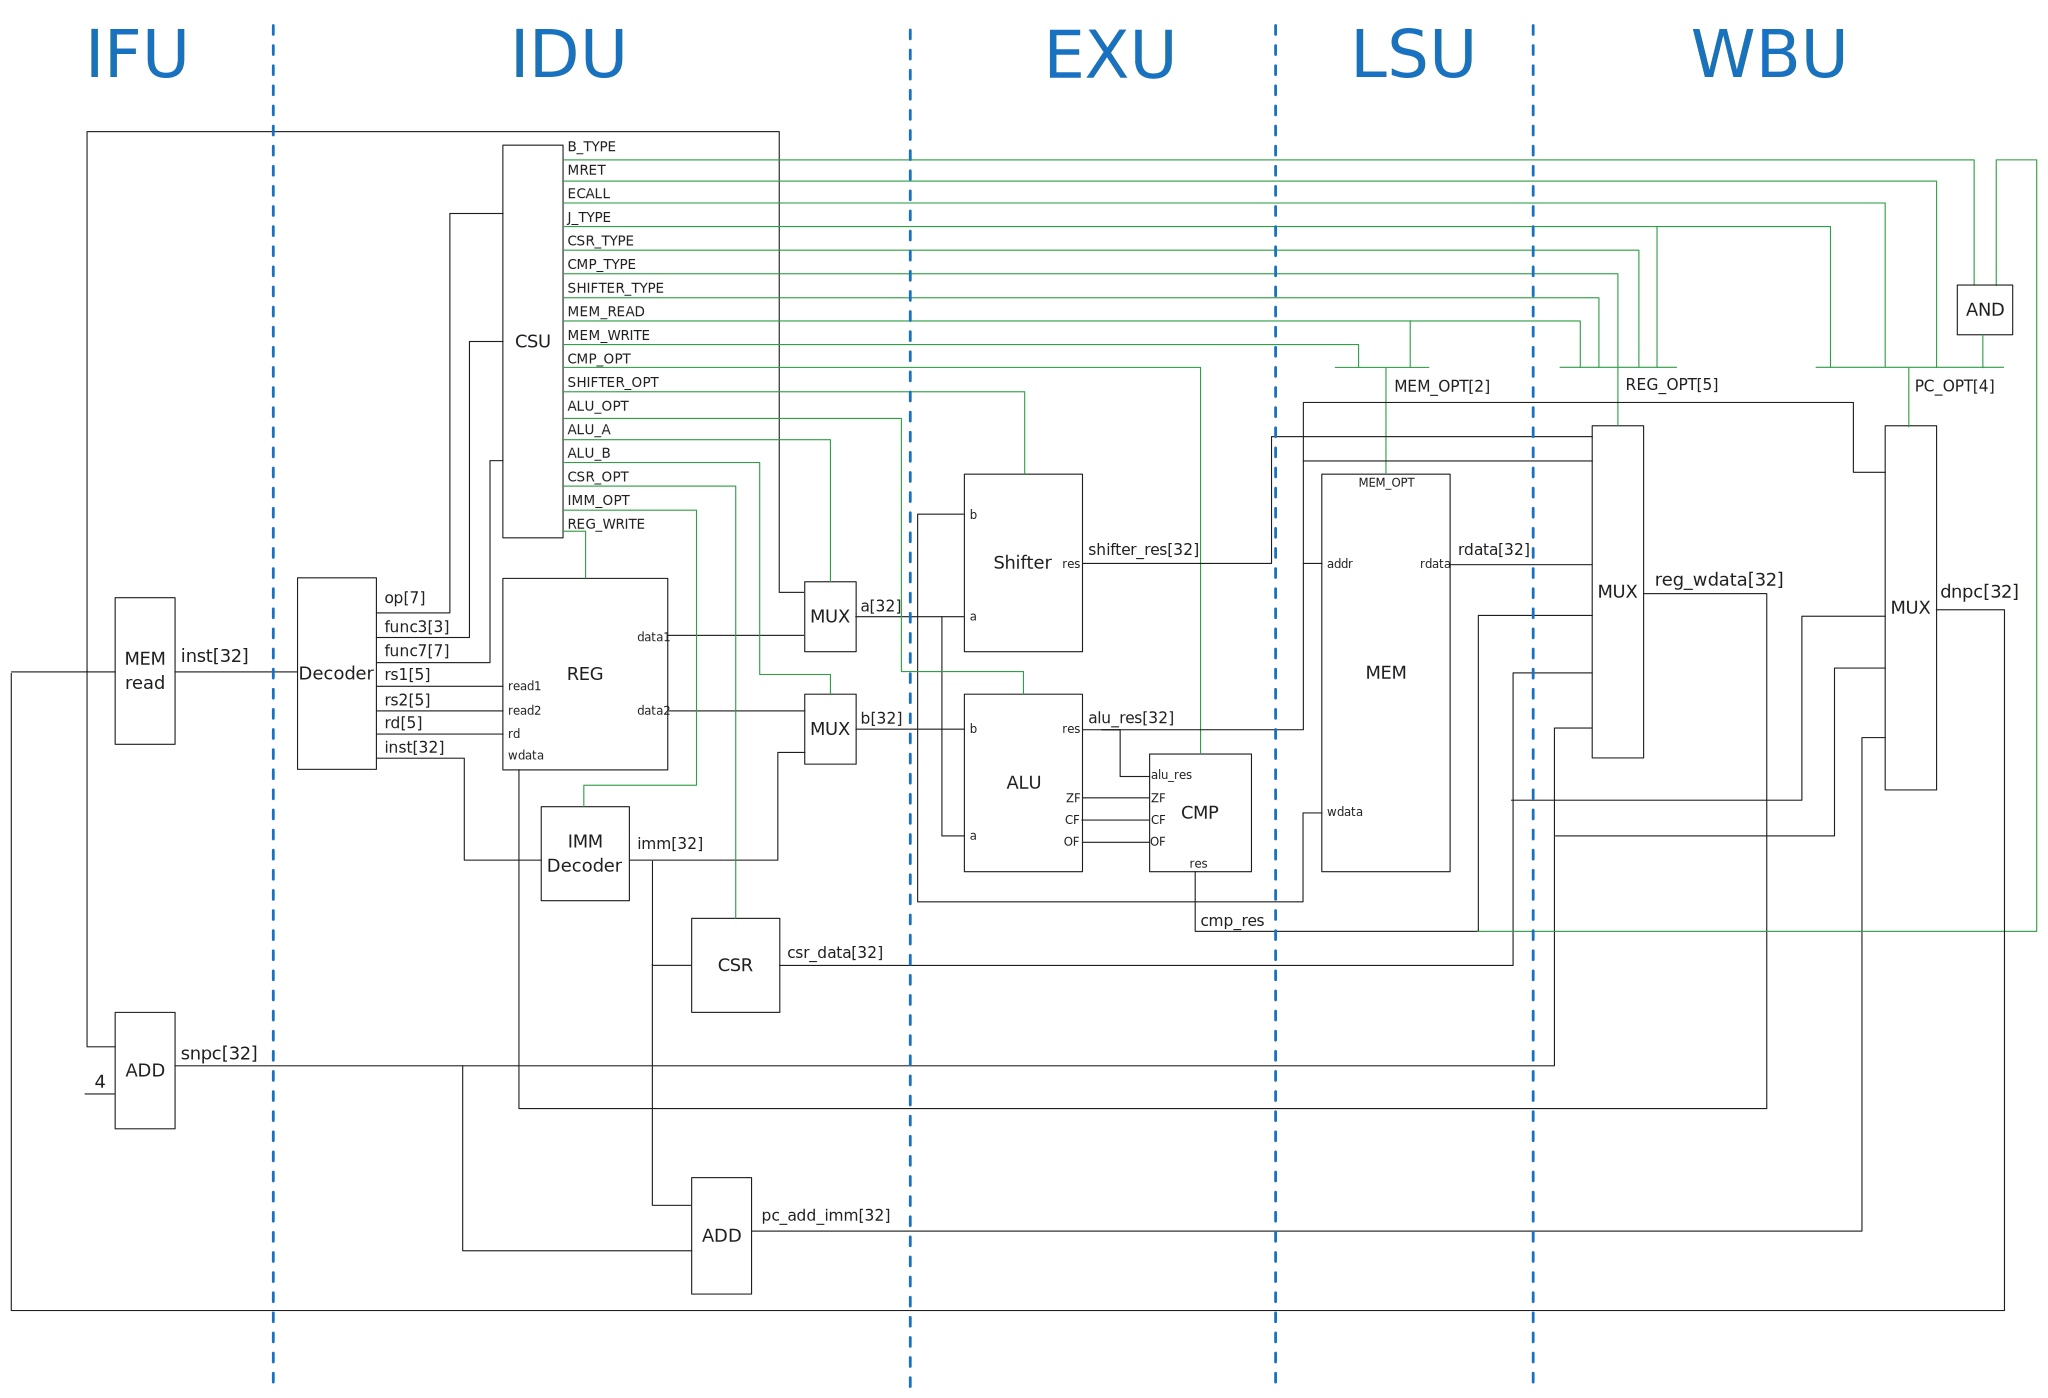
\includegraphics[width=1\textwidth]{image/cpu.pdf}
	\caption{处理器整体架构图}
	\label{fig:cpu}
\end{figure}

微处理器的整体架构如图\ref{fig:cpu}所示,主要由五个关键模块组成:IFU(取指模块)、IDU(译码模块)、EXU(执行模块)、LSU(访存模块)和WBU(回写模块)。以下是各模块的详细数据通路过程:

\begin{enumerate}
	\item \textbf{取指阶段}:取指模块根据PC(程序计数器)从内存中读取指令,并将指令传递给IDU。这一过程确保了指令流的连续性,为后续的处理步骤提供了基础。
	\item \textbf{译码阶段}:IDU负责将指令译码为多条控制信号。在这一阶段,寄存器的值被读取,同时进行立即数的符号扩展。译码后的控制信号被发送到EXU、LSU和WBU,以协调后续的执行和数据处理。
	\item \textbf{执行阶段}:EXU包含三个主要单元:加法器、移位器和比较器。这些单元根据来自IDU的控制信号执行算术和逻辑运算。运算结果随后被传递到EXU和WBU,以支持进一步的数据处理和存储。
	\item \textbf{访存阶段}:LSU根据来自IDU的控制信号和来自EXU的运算结果,执行存储器的读写操作。读取的数据被发送到WBU,以便后续的存储。
	\item \textbf{回写阶段}:WBU根据前面模块的信号,将处理结果写回到相应的寄存器中。这一阶段确保了数据的最终存储和状态的更新。
\end{enumerate}

通过这种模块化设计,微处理器能够高效地处理指令流,实现数据的快速通路。这种设计不仅展示了RISC-V架构的灵活性和高效性,还提供了一个深入了解计算机系统设计的机会。这种基于单周期设计的微处理器,为后续的多周期、流水线优化提供了十分便捷的基础。

\section{取指单元(IFU)}

\section{译码单元(IDU)}

\section{计算单元(EXU)}

\section{访存单元(LSU)}

\section{写回单元(WBU)}

\section{异常处理}




